%%%%%%%%%%%%%%%%%%%%%%%%%%%%%%%%%%%%%%%%%%%%%%%%%%%%%%%%%%%%%%%%%%%%%%
%%                     Trigger
%%%%%%%%%%%%%%%%%%%%%%%%%%%%%%%%%%%%%%%%%%%%%%%%%%%%%%%%%%%%%%%%%%%%%%

\subsection{Glyph: \glyph{Trigger}}\label{sec:trigger}
%\color{blue}

A trigger effect, or absolute stimulation, is a stimulation that is necessary for a process to take place. A process modulated by a trigger can only occur when this trigger is active.

\begin{glyphDescription}
 \item[SBO]\mbox{}\\ SBO:0000171 ! necessary stimulation
 \item[origin]\mbox{}\\ Any EPN (section~\ref{sec:EPNs}) or any logical operator (section~\ref{sec:logic}).
 \item[target]\mbox{}\\ Any transition node (section~\ref{sec:PNs}).
 \item[node]\mbox{}\\ The target extremity of a \glyph{trigger} carries an open arrow (to remind that it is a \glyph{stimulation}) coming after a larger vertical bar.
 \end{glyphDescription}

\begin{figure}[H]
  \centering
  \includegraphics[scale = 0.5]{images/trigger}
  \caption{The \PD glyph for \glyph{trigger}.}
  \label{fig:trigger}
\end{figure}

The example below describes the transcription of a gene X, that is the creation of a messenger RNA X triggered by the gene X. The creation of the protein X is then triggered by the mRNA X. (Note that the same example could be represented using the gene as reactant and product, although it is semantically different).

\begin{center}
\scalebox{0.5}{\includegraphics{examples/trigger-genetic}}
\end{center}

The example below describe the transport of calcium ions out of the endoplasmic reticulum. Without IP3 receptor, there is not calcium flux, therefore, one cannot use a \glyph{stimulation}. The trigger intead represents this absolute stimulation.

\begin{center}
\scalebox{0.5}{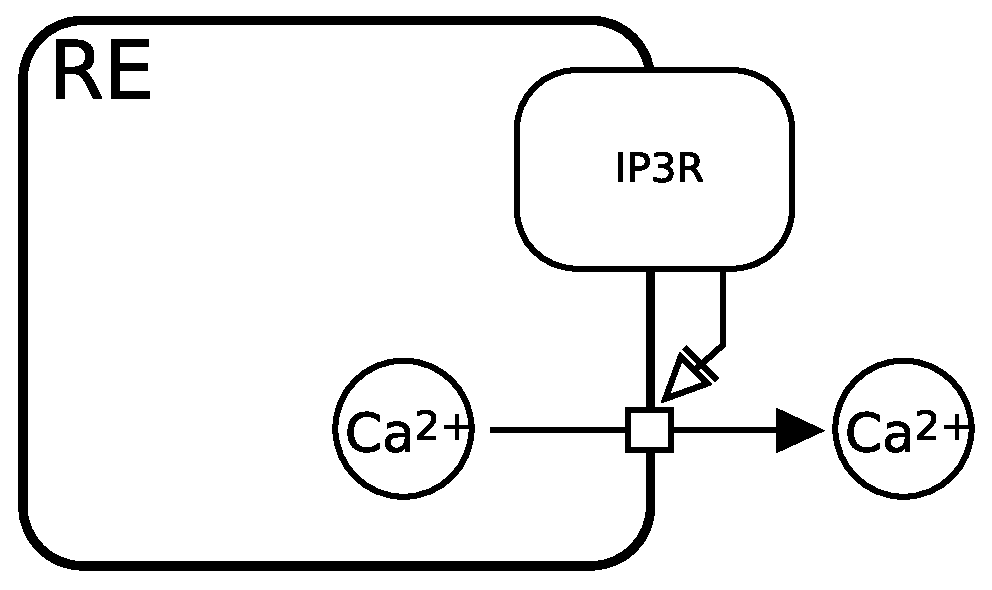
\includegraphics{examples/trigger-transport}}
\end{center}

\normalcolor

